\documentclass[../tfg.tex]{subfiles}

\begin{document}

\section{The heap}
The heap is a common term to refer to a portion of memory where programs can allocate memory at runtime for objects whom size is very large or unknown at compile time, and therefore, the compiler cannot manage the stack for them. This portion of memory is very often managed by libraries called allocators, in charge of keeping a record of the allocated and freed memory, its size, the possibility of reusing freed chunks and the merging of freed chunks to avoid heap fragmentation.

The C standard includes definitions for a set of heap functions common for everyone but the implementation is OS and library-dependent.

\begin{itemize}
    \item \texttt{malloc}
    \item \texttt{realloc}
    \item \texttt{calloc}
    \item \texttt{free}
\end{itemize}

\section{glibc malloc}
The GNU C malloc library contains implementations for the standard malloc functions, \texttt{malloc}, \texttt{free}, \texttt{realloc}, and \texttt{calloc}. This allocator manages the blocks of memory handled to a program in a "heap" style. The GNU malloc implementation is derived from ptmalloc (pthread's malloc) and in turn, ptmalloc derives from dlmalloc (Doug Lea's malloc).

\subsection{Common terms}

\subsubsection{Arena}
An arena is a region of memory dedicated to the allocator. Arenas hold references to one or more heaps from which they allocate and free memory. When a program is started, a main arena is created, that holds a reference to the initial heal. When more threads request allocations, more arenas can be created to avoid locking the main arena and causing a bottle-neck that could slow down the program.

\subsubsection{Heap}
Portion of memory reserved for allocations. This memory is subdivided into chunks handled by the allocator. Heap memory is contiguous, meaning that the are adjacent to one another.

\subsubsection{Chunk}
Subdivision of a heap. It is a block of memory with a certain size requested by the program. Chunks can be merged with neighboring chunks to obtain a larger chunk, or can be subdivided further to obtain smaller chunks, depending on the needs of the program.

When a chunk is freed, it gets pushed into a circular double-linked list called \textbf{bin}. To save up space, all the information required for the linked list management is stored on the chunk contents. This metadata includes forward and backward pointers and the size of the neighboring chunks. [\href{https://code.woboq.org/userspace/glibc/malloc/malloc.c.html#malloc_chunk}{\texttt{source code}}]

\begin{minipage}[c]{0.5\linewidth}
\begin{figure}[H]
    \centering
    \subfile{../imgs/heap_exploits/allocated_chunk_struct.tex}
    \caption{Allocated chunk structure}
    \label{fig:allocated_chunk_struct}
\end{figure}
\end{minipage}
\begin{minipage}[c]{0.5\linewidth}
\begin{figure}[H]
    \centering
    \subfile{../imgs/heap_exploits/freed_chunk_struct.tex}
    \caption{Freed chunk structure}
    \label{fig:freed_chunk_struct}
\end{figure}
\end{minipage}

\subsubsection{Tcache}
The Thread Local Cache is a special list of very recently freed chunks with the intention to be of quick access. It acts as a cache for freed chunks. Each thread owns a tcache containing a small collection of freed chunks for rapid access without the need to lock global variables or data structures like the arena, which is common for all threads under a process, to prevent data races.

The data structure is an array of bins, each bin being a linked list for chunks of certain sizes.

\begin{figure}[H]
    \centering
    \subfile{../imgs/heap_exploits/tcache_struct.tex}
    \caption{Tcache structure}
\end{figure}

This optimization is present from glibc version 2.26 upwards.

\section{Heap overflows}
Because chunks are contiguous in memory, we can overflow a heap buffer with more data than it can handle using unbounded write/read functions, just like a normal stack overflow.

\begin{figure}[H]
    \centering
    \subfile{../imgs/heap_exploits/heap_overflow.tex}
    \caption{Heap overflow}
    \label{fig:heap_overflow}
\end{figure}

\subsection*{Example}
To showcase this vulnerability I am going to solve the level \href{http://exploit.education/phoenix/heap-one/}{\emph{heap-one}} from \href{http://exploit.education/phoenix/}{\emph{Phoenix VM}}.

\begin{lstlisting}
struct heapStructure {
  int priority;
  char *name;
};

int main(int argc, char **argv) {
  struct heapStructure *i1, *i2;

  i1 = malloc(sizeof(struct heapStructure));
  i1->priority = 1;
  i1->name = malloc(8);

  i2 = malloc(sizeof(struct heapStructure));
  i2->priority = 2;
  i2->name = malloc(8);

  strcpy(i1->name, argv[1]);
  strcpy(i2->name, argv[2]);
  // ...
\end{lstlisting}

Thanks to the structures and the unbounded writes with the \texttt{strcpy} functions we can trigger an arbitrary write exploit. The second call to \texttt{strcpy} will take as a pointer \texttt{\&name} from the second struct. Because heap chunks are contiguous, the first \texttt{strcpy} call can keep writing data past the extent of \texttt{i1.name} into the second structure.

\begin{figure}[H]
    \centering
    \subfile{../imgs/heap_exploits/heap_overflow/heap_one.tex}
    \caption{heap-one@phoenix}
    \label{fig:heap_one_phoenix}
\end{figure}

We will use the first \texttt{strcpy} to override \texttt{i2.name} to point to another address where the value on the second argument will be written. In this case, I am overwriting it with the address of the return address on the stack and the second argument has the address of the \texttt{winner} function, performing a classical \texttt{ret2win} exploit but overriding data on the heap.

\begin{lstlisting}[caption={Pseudocode of the exploit}]
strcpy(&return_address, &winner);
\end{lstlisting}

\begin{figure}[H]
    \centering
    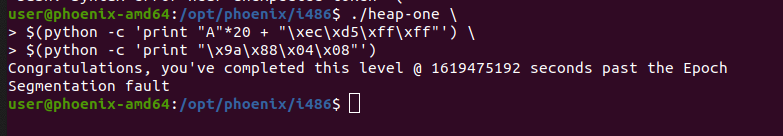
\includegraphics[width=\linewidth]{imgs/heap_exploits/heap_overflow/heap_one_solved.png}
    \caption{heap-one solved}
    \label{fig:heap_one_solved}
\end{figure}

\section{Use-After-Free}
An Use-After-Free vulnerability consists of the use of a chunk \textbf{after} it has been freed.

\begin{lstlisting}
#include <stdlib.h>
#include <string.h>

int main()
{
    char* buffer = malloc(sizeof(char) * 32);

    free(buffer);

    /* buffer still points to the chunk contents */

    memset(buffer, 0x41, sizeof(char) * 32);

    return 0;
}
\end{lstlisting}

\subsection*{Example}
To exemplify an UAF I will use \href{http://exploit.education/phoenix/heap-two/}{\emph{heap-two}} from \href{http://exploit.education/phoenix/}{\emph{Phoenix VM}}.

This program consist of a menu allowing us to perform some actions in arbitrary order over some global variables.
The program will check for the value of a variable inside the \texttt{auth} struct. By allocating and then freeing it we can force the following call to \texttt{malloc} returns us the same chunk that was allocated for the \texttt{auth} struct. Because the \texttt{auth} pointer is never cleared it points to the chunk that now belongs to the \texttt{service} variable, which we can control. By writing on \texttt{service} we are also writing on \texttt{auth}, therefore setting the correct value that the challenge expects to be completed.

\begin{figure}[H]
    \centering
    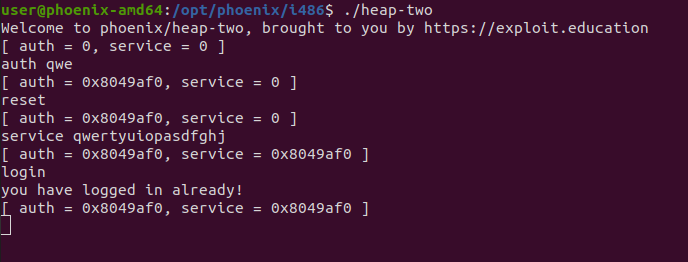
\includegraphics[width=\linewidth]{imgs/heap_exploits/use_after_free/heap_two_solved.png}
    \caption{heap-two@Phoenix}
    \label{fig:heap_two_phoenix}
\end{figure}

\section{Double free}
A double free consists of calling \texttt{free} two consecutive times on the same chunk. This causes a corruption on the allocator's data structures: the same chunk is appended two times to the free chunks list and the subsequent \texttt{malloc}s are going to return the same chunk to two different calls.

\begin{figure}[H]
    \centering
    \subfile{../imgs/heap_exploits/double_free_vuln.tex}
    \caption{Double free vulnerability}
    \label{fig:double_free_vuln}
\end{figure}

\subsection*{Example}
This is the \href{https://github.com/shellphish/how2heap/blob/master/glibc_2.31/fastbin_dup.c}{\texttt{fastbin\_dup.c}} exercise from \href{https://github.com/shellphish/how2heap}{\emph{how2heap}}

First, we allocate three chunks on the heap, \texttt{a, b} and \texttt{c}. Ideally, we only need one chunk: the other pointers are needed to bypass some security checks to prevent this kind of vulnerability.

\begin{figure}[H]
    \centering
    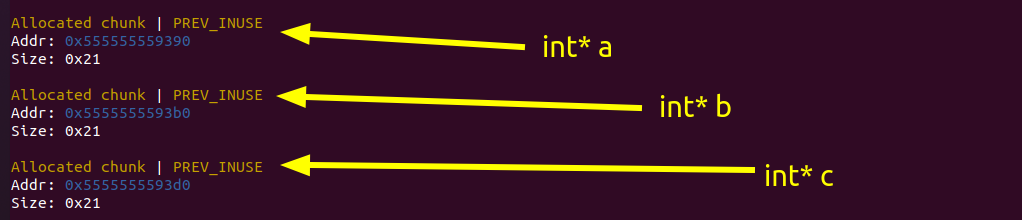
\includegraphics[width=\linewidth]{imgs/heap_exploits/double_free/double_free_1.png}
\end{figure}

Then, we free \texttt{a}.

\begin{figure}[H]
    \centering
    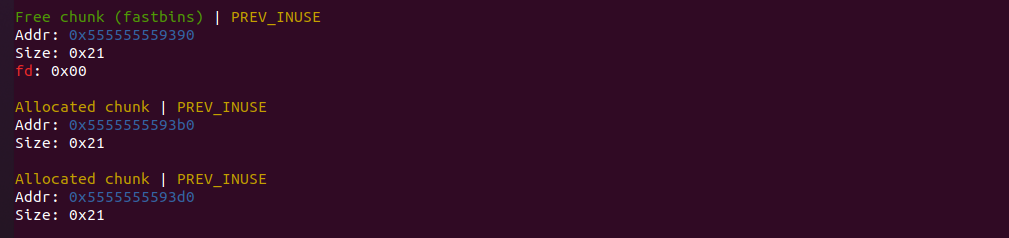
\includegraphics[width=\linewidth]{imgs/heap_exploits/double_free/double_free_2.png}
\end{figure}

Free \texttt{b} and then, again \texttt{a}. We have included \texttt{a}'s chunk two times on the bin.

\begin{figure}[H]
    \centering
    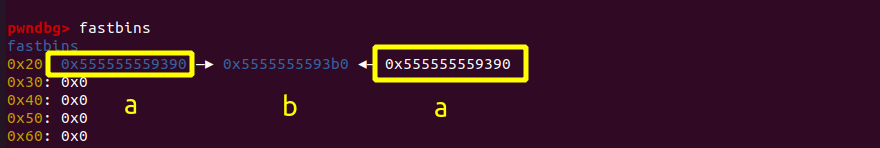
\includegraphics[width=\linewidth]{imgs/heap_exploits/double_free/double_free_3.png}
\end{figure}

Now the heap allocator is going to think they are two different chunks and hand them to two different \texttt{malloc} calls.

\begin{figure}[H]
    \centering
    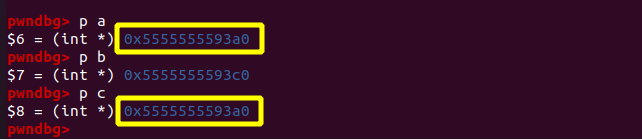
\includegraphics[width=\linewidth]{imgs/heap_exploits/double_free/double_free_4.png}
\end{figure}

Remember that the variables \texttt{a, b} and \texttt{c} points to the chunk contents, meanwhile the addresses shown in the fastbins are the addresses of the chunks.

\section{Unlink}
This attack exploits the \texttt{UNLINK} macro used in the \texttt{free} function. This macro executes the following instructions, redoing the connections between nodes on the double-linked list.
\begin{lstlisting}
#define unlink(P, BK, FD) {
    FD = P->fd;
    BK = P->bk;
    FD->bk = BK;
    BK->fd = FD;
}
\end{lstlisting}

\texttt{FD} and \texttt{BK} are pointers to the next and previous chunk of \texttt{P}. If the attacker can control the chunk to be unlinked, \texttt{P}, we can put arbitrary values on \texttt{FD} and \texttt{BK}.

Imagine the following setup:

\begin{figure}[H]
    \centering
    \subfile{../imgs/heap_exploits/unlink/controlled_chunk.tex}
    \caption{User controlled chunk}
\end{figure}

Following the \texttt{unlink} macro execution:\\

\begin{centering}
\texttt{FD} $=$ \texttt{0x5655d804}\\
\texttt{BK} $=$ \texttt{0x5508f311}\\
*(\texttt{0x5655d804} $+$ \texttt{0xc}) $=$ \texttt{0x5508f311}\\
*(\texttt{0x5508f311} $+$ \texttt{0x8}) $=$ \texttt{0x5655d804}\\
\end{centering}

\vspace{15pt}

That is an arbitrary write. The values on \texttt{FD} and \texttt{BK} should take in account the offset on the struct. For example, \texttt{FD} should point to an address \texttt{0xc} bytes lower than the actual address we want to write to.

Newer glibc versions patched this exploit by adding sanity checks for the chunk headers. This exploit no longer works on the newer glibc versions.

\end{document}
